\documentclass[10pt,twocolumn]{article}



\usepackage[utf8]{inputenc}
\usepackage{amsmath}
%\usepackage{ae}
\usepackage{graphicx}
\usepackage{color}
%\usepackage{bbm}
%\usepackage[swedish]{babel}
\newcommand{\N}{\ensuremath{\mathbbm{N}}}
\newcommand{\Z}{\ensuremath{\mathbbm{Z}}}
\newcommand{\Q}{\ensuremath{\mathbbm{Q}}}
\newcommand{\R}{\ensuremath{\mathbbm{R}}}
\newcommand{\C}{\ensuremath{\mathbbm{C}}}
\newcommand{\rd}{\ensuremath{\mathrm{d}}}
\newcommand{\id}{\ensuremath{\,\rd}}
\newcommand{\ket}[1]{|#1\rangle}
\newcommand{\bra}[1]{\langle#1|}
\newcommand{\braket}[2]{\bra{#1}#2\rangle}
\newcommand{\bracket}[3]{\bra{#1}#2\ket{#3}}

\title{Speed and Lifetime Measurement of Cosmic Muons}
\author{Jonathan Lindgren \and Petter Säterskog}
\newpage
\usepackage[margin=2.0cm]{geometry}
\begin{document}
\twocolumn[
  \begin{@twocolumnfalse}
    \maketitle
    \begin{abstract}
      The speed and lifetime of cosmic muons have beem measured. The speed measurement was done using two scintillation detectors and a gamma source. The speed $0.99c\pm$ was obtained by optimizing a Monte-Carlo model of the setup with four free parameters. The lifetime measurement was done by slowing down muons in a large scintillation detector and measuring the time between the slowing down and the decay. A maximum likelihood estimator was used for the lifetime and a noise as parameters of the probability density function.
    \end{abstract}
  \end{@twocolumnfalse}
  ]
Cosmic muons are created by energetic particles hitting the upper atmosphere. Muons are charged leptons 200 times heavier than the electron. Cosmic muons lose energy through bremsstrahlung when travelling through matter but muons penetrate long distances due to their large mass\cite{PhysRevD.45.3051}. Muons decay into leptons of lower mass and have a lifetime of about 2$\mathrm{\mu s}$ but they live longer in our frame of reference due to relativistic time dilation\cite{frisch:342}. We have made two experiments, a speed measurement of cosmic muons and a lifetime measurement of muons.\\
Our setup consist of three plastic scintillation detectors located on top of each other. The upper two detectors, P$_1$ and P$_2$, are flat. They are separated by a gap of 2.4 meters with P$_1$ on the top. The lowest detector, B, was bigger to be able to fully stop the muons. When a muon goes through one of the detectors we will get a light pulse that is amplified by a photo multiplier tube (PMT). The time difference between pulses from P$_1$ and P$_2$ can be used for determining the speed of the muons. These PMT signals were reshaped by a constant fraction discriminator (CFD) and then sent to a time to amplitude converter (TAC). The signal from P1 was used to start the TAC and the signal from P$_2$ to stop it. See Fig. \ref{setup}. A computer recorded the output of the TAC. The relationship between the channel recorded by the computer and the time delay measured by the TAC was determined by sending pulses of known delays to its start and stop inputs.\\  %ev bild av tCal
The difference of the delays of the signals from P$_1$ and P$_2$ to the start and stop of the TAC, $\Delta t$, is not known due to the possible differences in the PMTs and cabelings. A radioactive $^{60}$Co sample was placed below P$_2$ for calibration. It releases two photons simultaneously so that they can be detected in both P$_1$ and P$_2$. The pulses from P$_2$ were delayed enough for both the muons going through P$_1$ and then P$_2$ and the photons going the opposite direction to be timed by the TAC. Plotting the measured times as a histogram shows two peaks, see Fig. \ref{speedHist}. A constant noise measured at the end of the interval has been removed from the measurement data.
\begin{figure}
\centering
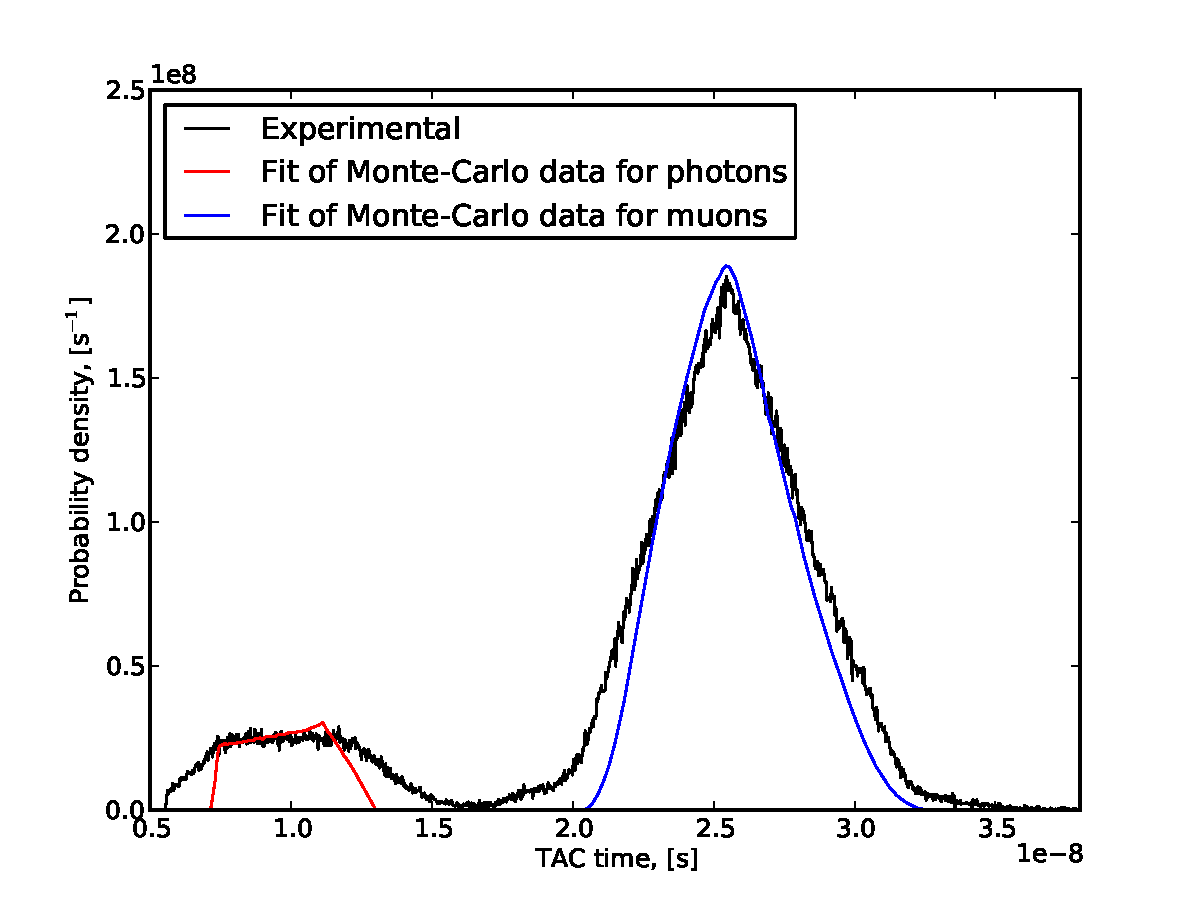
\includegraphics[width=8.6cm]{speedFit.pdf}
\caption{Histogram of time measured by TAC in speed measurement.}
\label{speedHist}
\end{figure}
The first peak is from the photons and the later from the muons. The shape and position of the photon peak in the spectrum can be calculated from $\Delta t$ and the geometry of the setup. The dimensions of the setup were measured and a Monte-Carlo (MC) simulation was performed. The photons were assumed to move straight to the PMT in the scintillating material with index of refraction 1.50. The detectors were modeled as two dimensional polygons, see Fig. \ref{MC}.
\begin{figure}
\centering
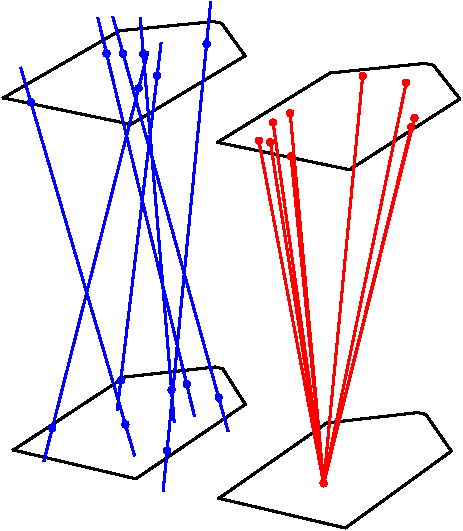
\includegraphics[width=5cm]{mc-crop.pdf}
\caption{Some samples from the MC simulation of the speed measurement. The blue lines are muon tracks and the red lines are photon tracks. Dots indicate interactions with the detector.}
\label{MC}
\end{figure}
$\Delta t$ was obtained by minimizing
\begin{equation}
 \mathrm{err}_\gamma(\Delta t, N_\gamma)=\int\mathrm{d}t\left(f_{\gamma,\mathrm{exp}}(t)-N_\gamma f_{\gamma,\mathrm{MC}}(t-\Delta t)\right)^2
\end{equation}
where $f_{\gamma,\mathrm{exp}}(t)$ is the experimental distribution of delays and $f_{\gamma,\mathrm{MC}}(tt-\Delta t)$ is the probability distribution obtained from MC simulations. The position and shape of the muon peak can in the same way be calculated using MC methods using the value of $\Delta t$, see Figure \ref{MC}. The peak shape and position now both depend on the speed distribution of the particles. All muons are assumed to have the same speed $v$ and having a uniform angular distribution in the range measured, less then $29^\circ$ from vertical. The speed $v$ can be varied to find the best fit to experimental data by minimizing
\begin{equation}
 \mathrm{err,N_\mu}_\mu(v)=\int\mathrm{d}t\left(f_{\mu,\mathrm{exp}}(t)-N_\mu f_{\mu,\mathrm{MC}}(t,v)\right)^2
\end{equation}
where $f_{\mu,\mathrm{exp}}(t)$ is the experimental distribution of delays and $f_{\mu,\mathrm{MC}}(t,v)$ is the probability distribution obtained from MC simulations using muon speed $v$. The speed $2.9783\cdot10^8$m/s was obtained. This result contains systematic errors from assuming uniform muon angular distribution and uniform muon speed. Using an angular distribution peaked at vertical muons give a more peaked histogram in Figure \ref{speedHist}. Using a speed distribution would make the peak wider in Figure \ref{speedHist}. This might account for the discrepancy seen between experiment and MC for this peak. The errors in the widths of the peaks are of order 1 ns so this can be the expected order of the systematic errors. This gives the order of the systematic errors in the velocity to 10\%. There is also a statistical error of 5mm in the height measurement. This gives a statistical error in the result of 0.2\%. The statistical errors from the finiteness of the sample and the MC sample are negligible compared to the systematic errors.\\

The muons energy and thus $\gamma$-factor is unknown so they need to be slowed down to non-relaivistic speeds for a lifetime measurement. To determine the lifetime of the muons we used on scintillator and the barrel detector. Coincidence between the barrel and the scintillator were used to be able to identify signals from muons that went through the scintillator and then absorbed in the barrel. The barrel will first give a signal from the energy absorbed when slowing down the muon and another signal when it decays. The start and stop signals are separated by an AND respectively AND-NOT gate with the scintillator signal, see fig().

To determine the lifetime of the muon we fitted an exponential distribution to the measured data. However, the Time To Amplitude converter could not measure very well for small and large lifetimes, thus we only considered a limited interval $[t_1,t_2]$ and this has to be taken into account into the propability distribution. By looking at the spectrum it is reasonable to also add a constant noise $C$, so the distribution is
\begin{equation}
f(t)=\frac{\exp{(-t/\tau)}+C}{\tau\exp{(-t_1/\tau)}-\tau\exp{(-t_2/\tau)}+C(t_2-t_1)}\label{pdf}
\end{equation}

To determine $\tau$ and $C$ for our measured data the likelyhood function $\prod f(t_i)$ was minimized yielding $\tau=2.0$ $\mu$s and $C=0.05$. \newline

The statistical error was determined by sampling many different simulated sets of data points by using the distribution \eqref{pdf} and then calculate the standard deviation of these sets. The likelyhood function was also calculated to see that it was consistent with the likelyhood function for the real data points, thus verifying the validity of the model. \newline

By applying the same method it is also possible to verify that the obtained constant noise is not just statistical fluctuations. Minimizing the likelyhood function with respect to the lifetime and the constant noise set to zero a lifetime of $2.21$ $\mu$s is obtained. Using this lifetime to sample new sets of data points, and then fitting the distribution \eqref{pdf} to these data points it is possible to obtain the expected size of the statistical noise. This gives a simulated mean noise of $1.3\cdot 10^{-4}$ with standard deviation $9.4\cdot 10^{-5}$ compared to the noise of the data which is about $0.0021$. It is thus clear that this can not be explained by statistical fluctuations and must be taken into account in the model.

The muon speed is hard to measure using only two detectors. Larger scintillator separation could be used for increased accuracy of the parameter fit. A more vertical measurement with sharper peak in Fig. \ref{speedHist} would then be obtained. This would require increased time of measurement. A distribution of speeds could be obtained if the MC model is more accurate. The muon speed is very close to $c$ so an energy measurement would be much more efficient than our approach if the muon mass is known.\\

The obtained lifetime for the muon is slightly lower than the accepted value of $2.2$ $\mu$s which is not even in our error margin. However, this can be explained by the fact that there are two muons, $mu^+$ and $\mu^-$, which doesnt have the same lifetimes in the detector material \cite{}. $\mu^+$ has the same lifetime as in vacuum, while $\mu^-$ has a lifetime of about $2.0$ $\mu$s. The size of the measurement data obtained in this experiment is too small to be able to separate these two exponential distributions.
\\

The authors would like to thank Ronja Thies for her support.
% Figurer inkluderade som eps-filer
%% \begin{figure}\centering
%% 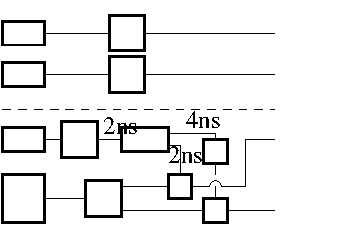
\includegraphics{speed.pdf}
%% \caption{\label{figuren} Perioden $T$ som funktion av pendellängden.}
%% \end{figure}

% Figurer inkluderade med xfigs postscript+latex

\begin{figure}[h]
\input{speed.pspdftex}
\caption{\label{setup} Schematic diagram of the different operations acting on the input signals.}
\end{figure}
\bibliographystyle{plain}
\bibliography{report}
\end{document}
